\section*{Introduction}
 The algorithms and methods discussed in the previous chapters for preprocessing and feature extraction are implemented and compared using Physionet dataset, BBCI dataset and the data collected from OpenBCI headgear. This chapter discusses about the results obtained from BCI signal processing pipeline combining different preprocessing, feature extraction and classification algorithms. Several open source libraries were used in BCI data extraction, analysis and visualization.

\section{Preprocessing}
 The EEG data recorded from the OpenBCI headgear is given in the figure \ref{fig:obci_rawfltrd}. The figure represents data that is free from power line noise and the frequency is limited to the frequency of interest. The colored lines on the plot mark the onset of the event with the number on the top representing the event ID. The event markers are used in setting baseline and transforming raw data into epochs. Teh electrode locations are given in the figure \ref{fig:obci_eegpose}.

 \begin{figure}[h]
    \begin{center} 
    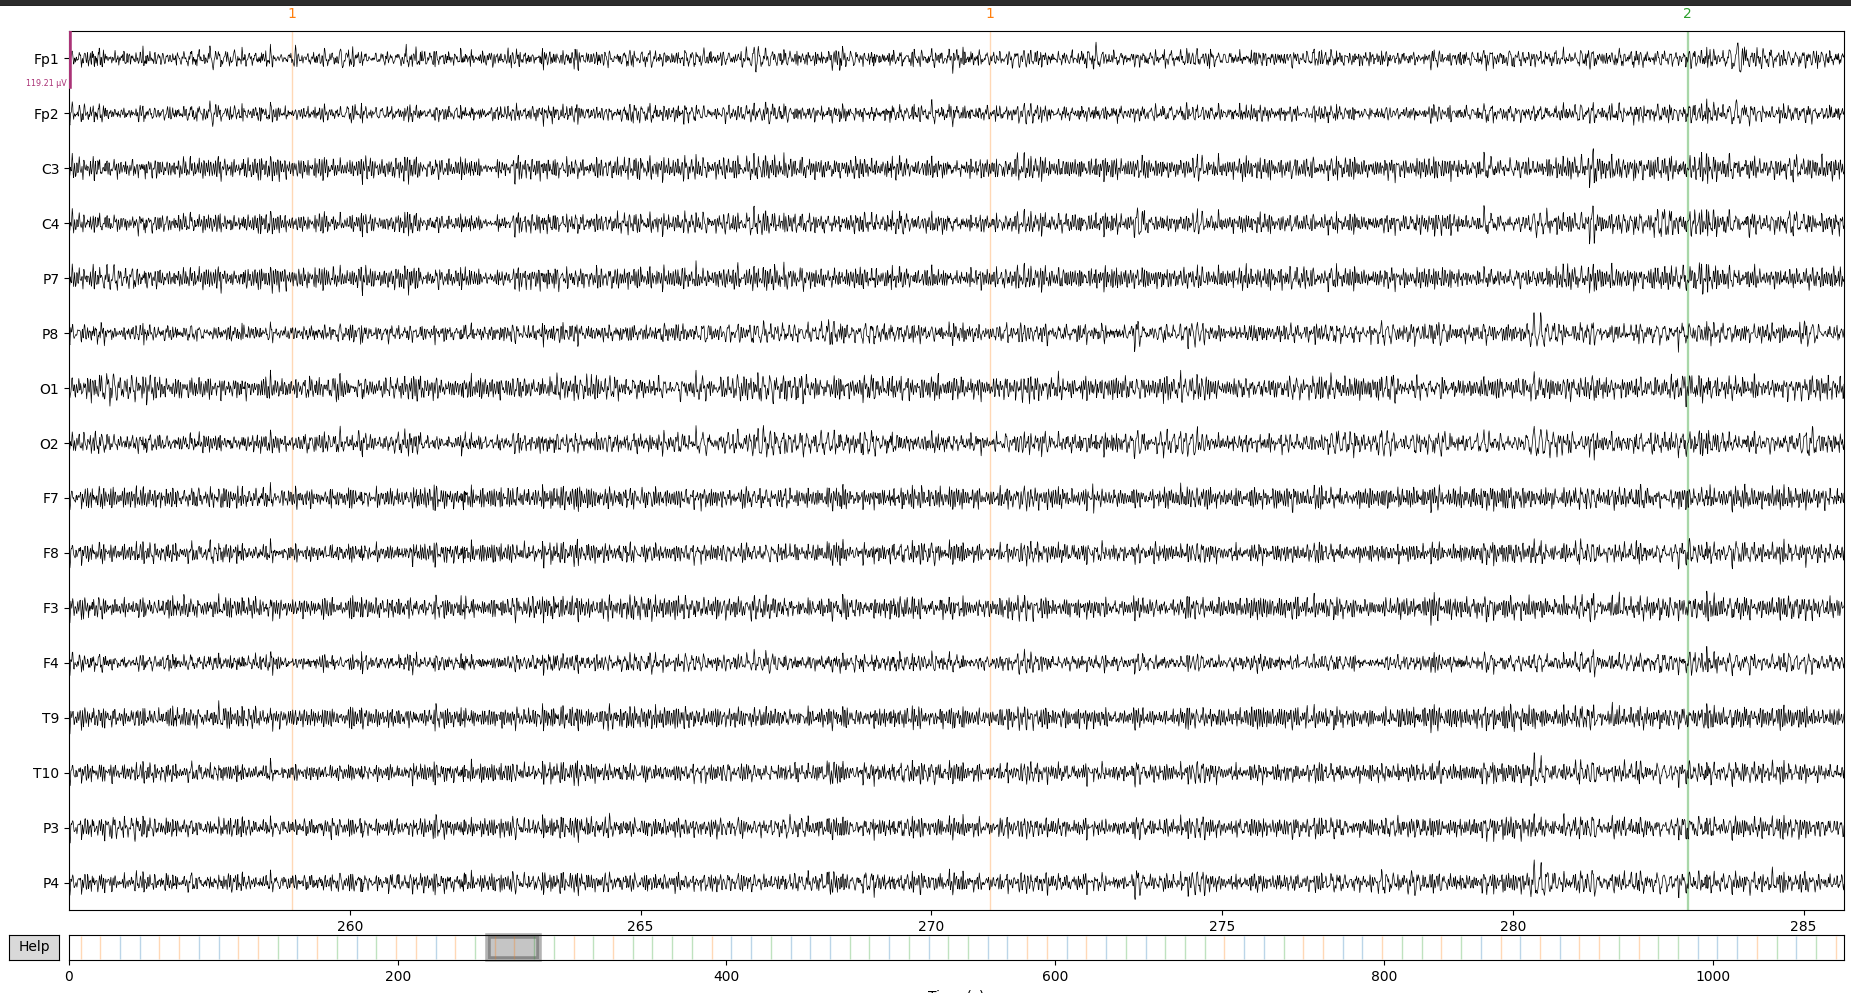
\includegraphics[height=0.6\textwidth]{images/obci_rawfltrd.png}
    \caption{Raw data(filtered) captured from OpenBCI headgear}
    \label{fig:obci_rawfltrd}
\end{center}
\end{figure}

\begin{figure}[h] 
    \begin{center}
    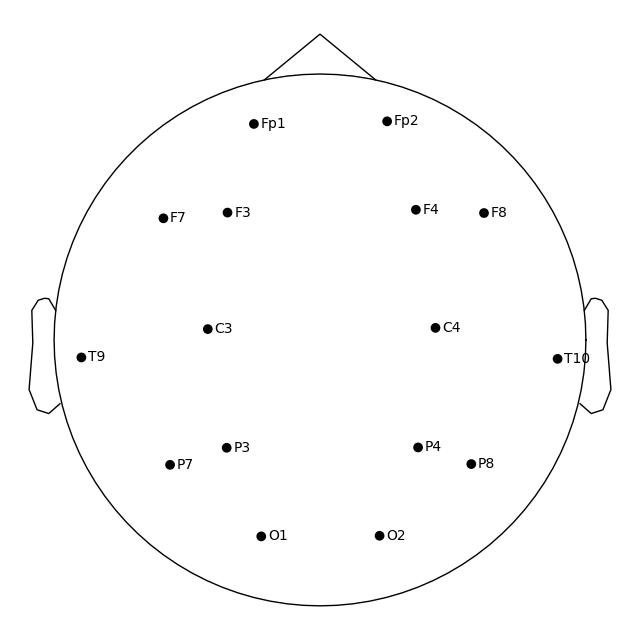
\includegraphics[height=0.6\textwidth]{images/obci_eegpose.png}
    \caption{}
    \label{fig:obci_eegpose}
\end{center}
\end{figure}


 The frequency contents of the filtered raw data is given in the picture \ref{fig:obci_rawfltrd_psd}. The color scheme represents the location of the electrodes. In a normal indoor experimental setup the OpenBCI hardware tends to pick up several noisesfrom the surrounding and hence a peak is observed at 25Hz. This does not appear in case of OpenBCI dataset \ref{fig:phy_rawfltrd_psd} as the recordings were made in a laboratory environment.

\begin{figure}[h] 
    \begin{center}
    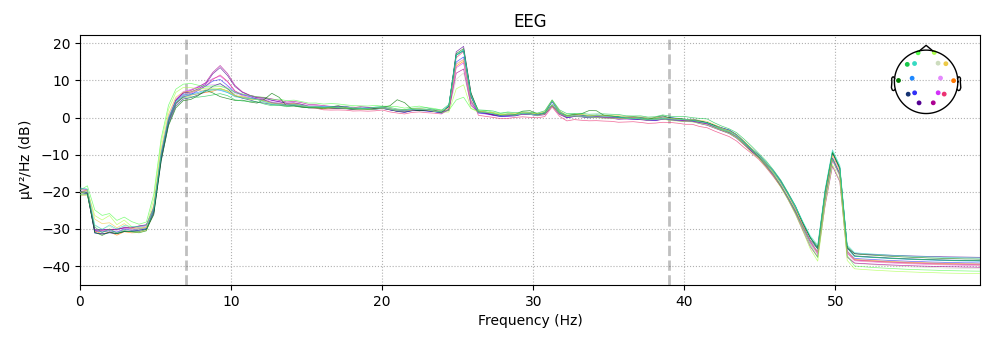
\includegraphics[height=0.6\textwidth]{images/obci_rawfltrd_psd.png}
    \caption{}
    \label{fig:obci_rawfltrd_psd}
    \end{center}
\end{figure}

\begin{figure}[h] 
    \begin{center}
    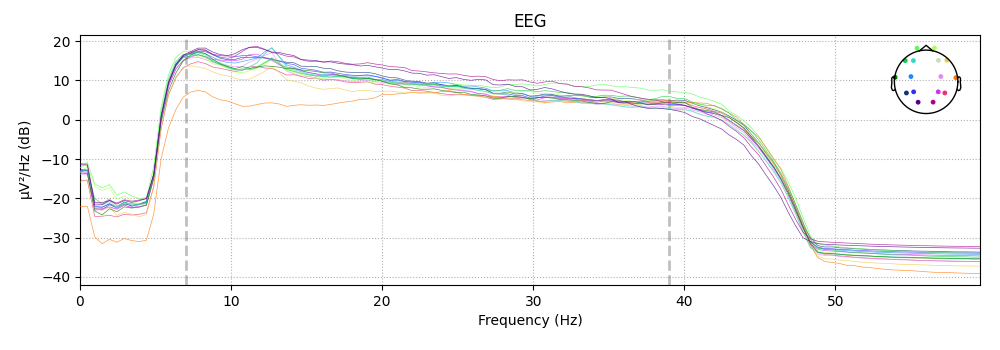
\includegraphics[height=0.6\textwidth]{images/phy_rawfltrd_psd.png}
    \caption{}
    \label{fig:phy_rawfltrd_psd}
\end{center}
\end{figure}

From the filtered raw data only frequency region of intrest i.e. Beta and the Gamma band is used in further analysis. Based on the frequency band of interest, the topography is given in \ref{fig:obci_psd_topomap}

\begin{figure}[h] 
    \begin{center}
    \includegraphics[height=0.6\textwidth]{images/obci_psd_topomap.png}
    \caption{}
    \label{fig:obci_psd_topomap}
\end{center}
\end{figure}

With common average referencing \ref{fig:obci_car}
\begin{figure}[h] 
    \begin{center}
    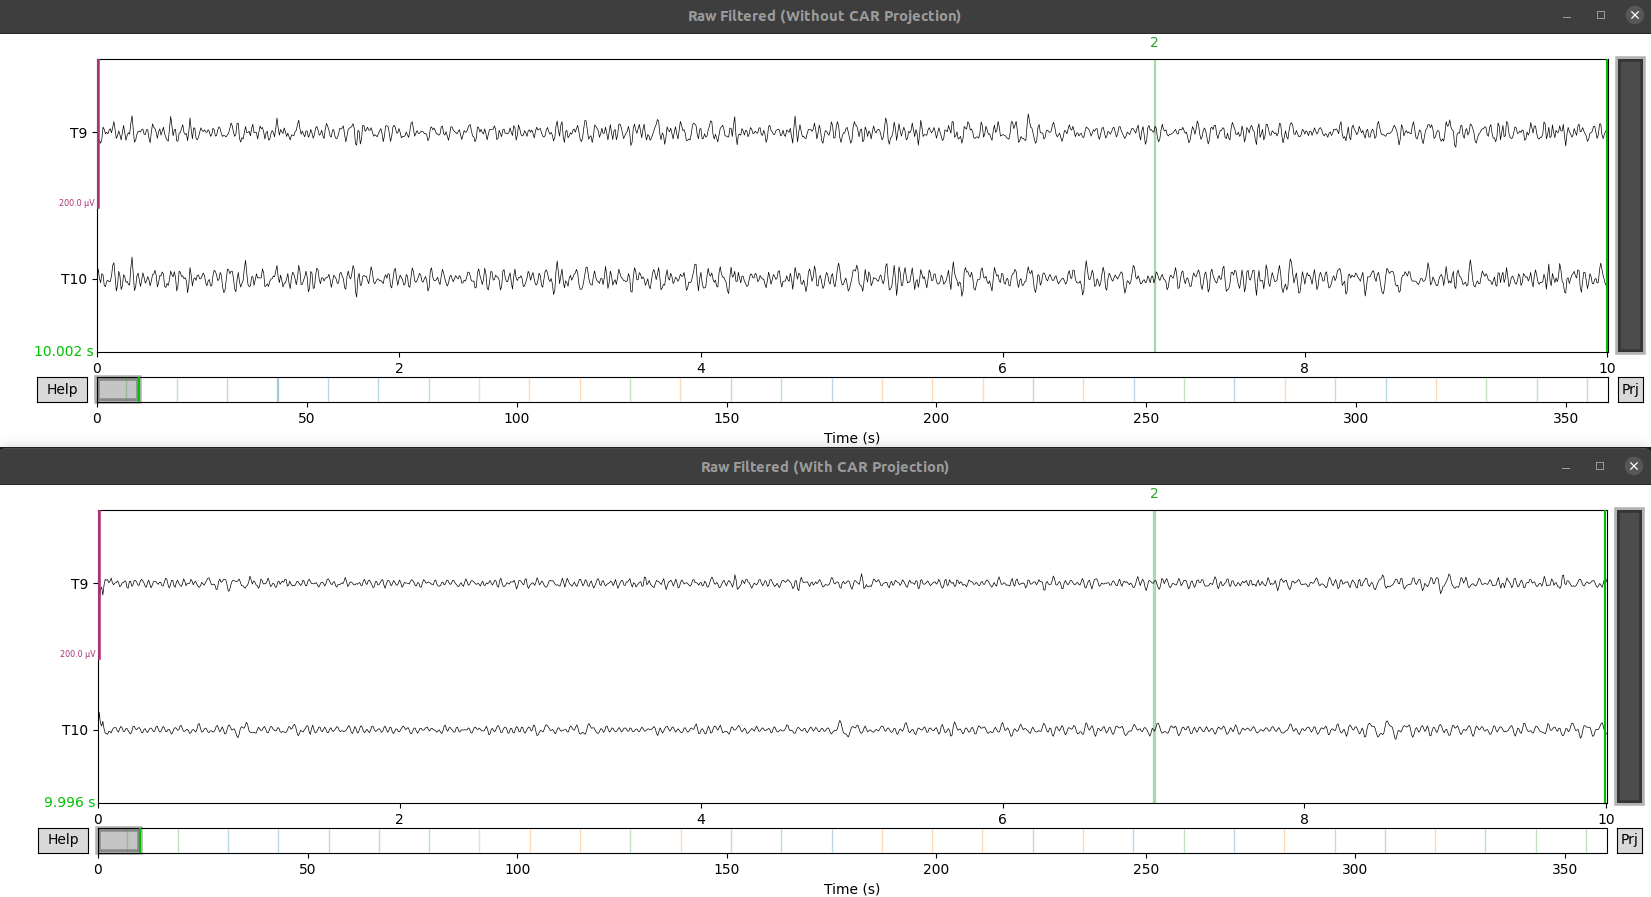
\includegraphics[height=0.6\textwidth]{images/obci_car.png}
    \caption{}
    \label{fig:obci_car}
\end{center}
\end{figure}

With signal space projection \ref{fig:obci_ssp}
\begin{figure}[h] 
    \begin{center}
    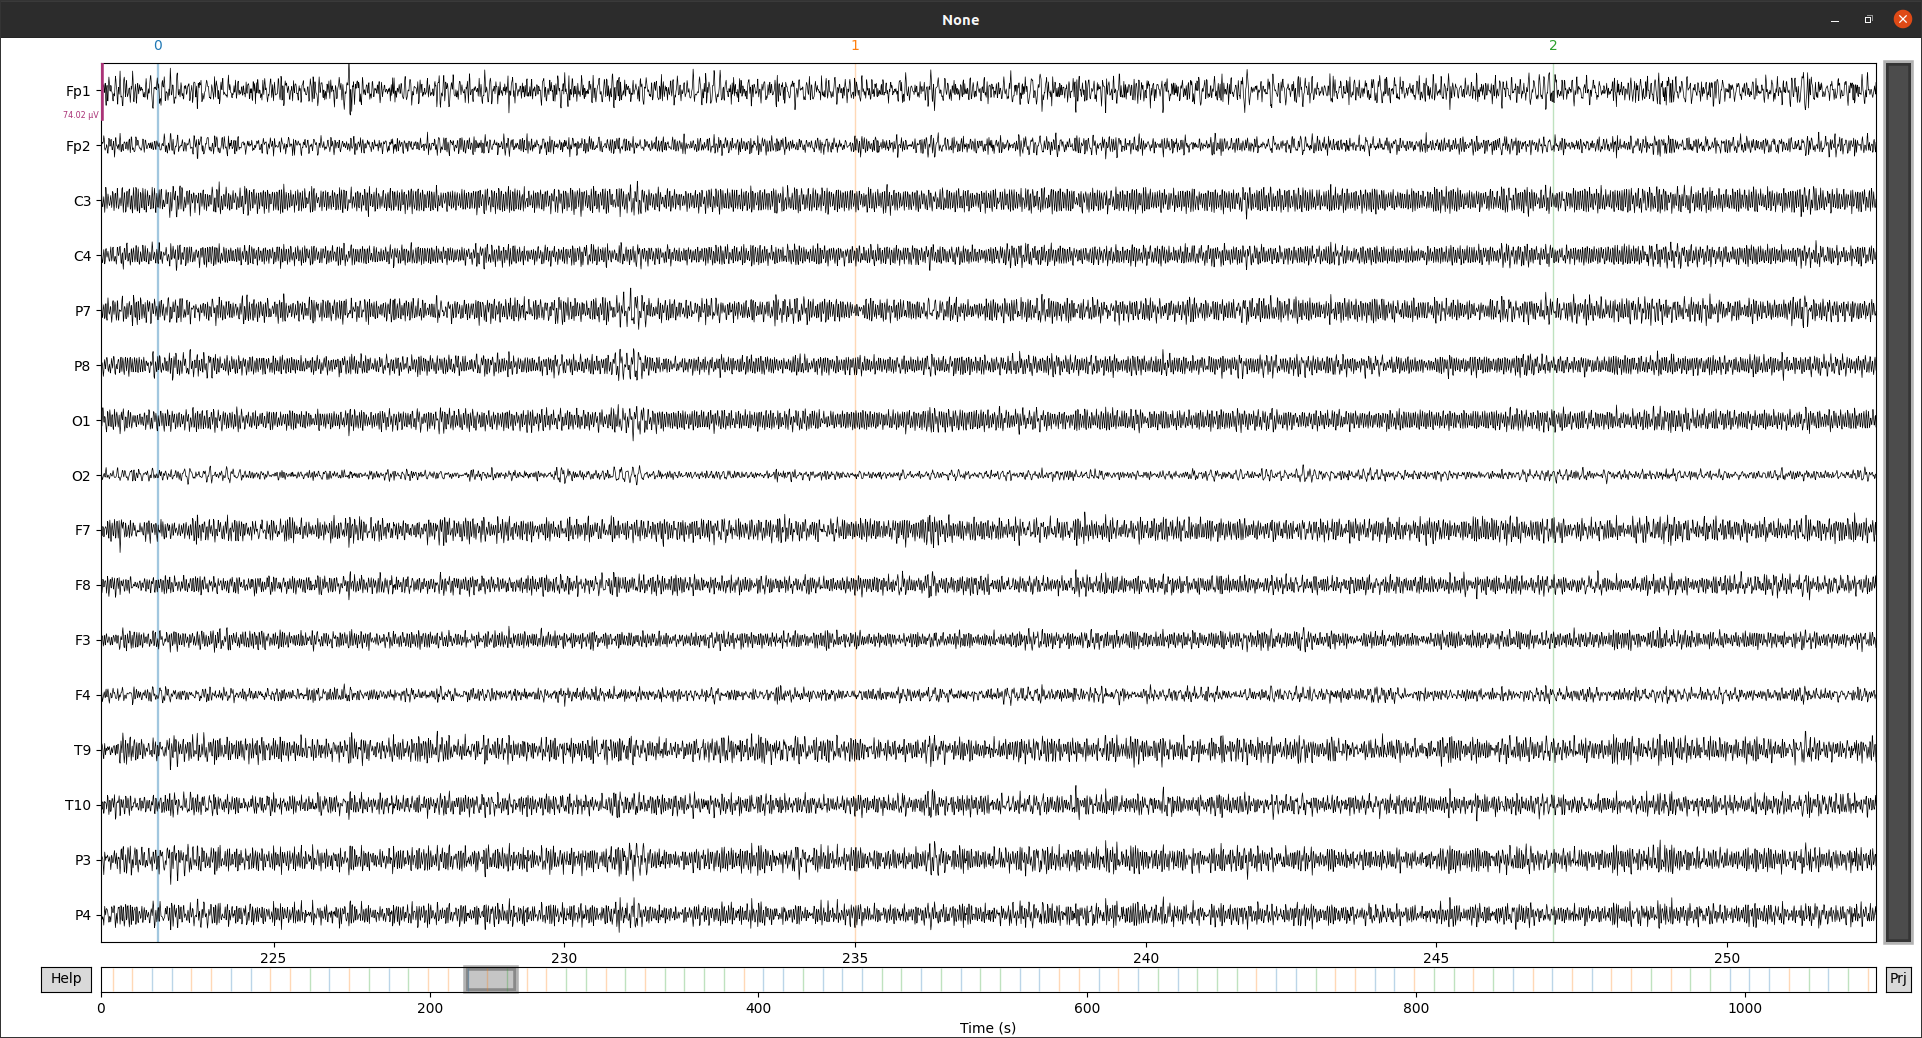
\includegraphics[height=0.6\textwidth]{images/obci_ssp.png}
    \caption{}
    \label{fig:obci_ssp}
\end{center}
\end{figure}

ICA removes the noisy components in the raw data 

Fig : 1, Raw
2, psd topography
3, ICA - ocerlay
4, ICA - Sources
5, ICA - Scores
6, ICA - Prop
7, ICA - Components
8, SSP - projmap
9, SSP - Raw
10, CAR - projmap
11, CAR - Raw
12, Epoch Image
13, topography
14, Evoked data
15, white noise
16, CSP - plot_patterns

\section{Spatial Information}

\section{Temporal Information}

\section{Spatio-Temporal Information}

\section*{Summary}